% SCA method diagram (Figure~\ref{fig:method}), built at ICLR text width (5.5 in = 397.48 pt).
% Compile from the project root:
%   tectonic -o paper/figures paper/figures/src/method_sca.tex   (writes paper/figures/method_sca.pdf)
% Palette: blue = image-anchored branch (O^glob), green = pixel-anchored branch (O^loc),
% vermillion = the contribution (calibrated per-head mix). Everything else is neutral grey.

\documentclass[border=0pt]{standalone}
\usepackage{tikz}
\usepackage{amsmath}
\usetikzlibrary{arrows.meta, positioning, fit, backgrounds, calc, shapes.geometric}

\newcommand{\Oloc}{O^{\mathrm{loc}}}
\newcommand{\Oglob}{O^{\mathrm{glob}}}
\newcommand{\Ofull}{O^{\mathrm{full}}}
\newcommand{\pih}{\pi_{h}(\sigma)}

\definecolor{cglob}{HTML}{0072B2}
\definecolor{cloc}{HTML}{009E73}
\definecolor{cacc}{HTML}{D55E00}

\tikzset{
  orx/.style={
    font=\sffamily\footnotesize,
    >={Stealth[round, length=4pt, width=3pt]},
    line width=0.5pt,
    node distance=4mm and 6mm,
  },
  block/.style={
    draw=black!55, fill=white, rounded corners=1pt,
    minimum height=6.5mm, inner sep=2.5pt, align=center,
  },
  glob/.style={block, draw=cglob!85, fill=cglob!8},
  loc/.style={block, draw=cloc!85, fill=cloc!8},
  skipped/.style={block, draw=black!30, dashed, fill=white, text=black!45},
  ours/.style={block, draw=cacc, fill=cacc!8, line width=0.8pt},
  muted/.style={block, draw=black!35, fill=black!3},
  data/.style={
    draw=cacc, fill=cacc!8, line width=0.8pt, trapezium, trapezium left angle=72,
    trapezium right angle=108, trapezium stretches body,
    minimum height=6mm, inner sep=2pt, align=center,
  },
  flow/.style={->, draw=black!65},
  accflow/.style={->, draw=cacc, line width=0.8pt},
  edgelbl/.style={font=\sffamily\scriptsize, text=black!65, inner sep=1pt, fill=white},
  stage/.style={draw=black!30, dashed, rounded corners=2pt},
  stagelbl/.style={font=\sffamily\scriptsize, text=black!70, inner sep=0pt, anchor=north west},
  panel/.style={font=\sffamily\footnotesize, inner sep=0pt, anchor=north west},
  note/.style={font=\sffamily\scriptsize, text=black!75, align=center, inner sep=0pt},
}

\begin{document}
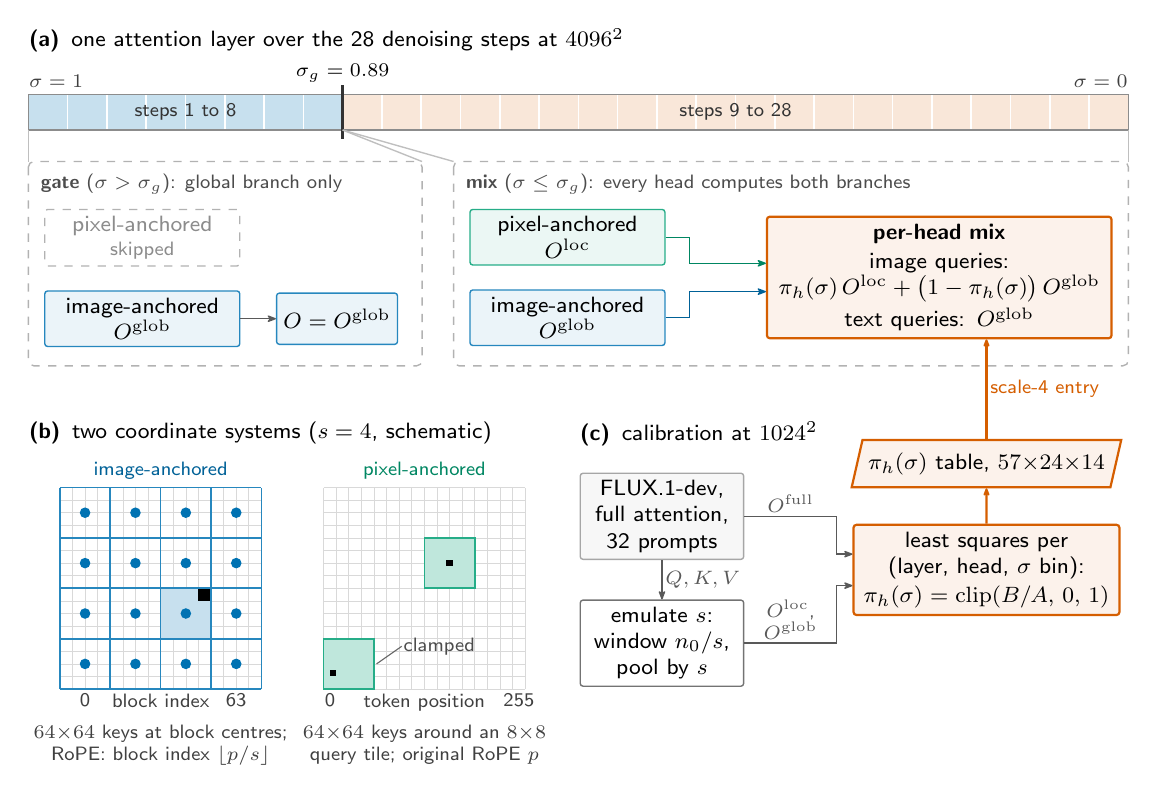
\begin{tikzpicture}[orx, x=1mm, y=1mm]

  \pgfmathsetmacro{\W}{139.7}
  \pgfmathsetmacro{\cw}{\W/28}

  % =====================================================================
  % (a) Denoising pipeline
  % =====================================================================
  \node[panel] at (0,0) {\textbf{(a)}\, one attention layer over the 28 denoising steps at $4096^2$};

  % timeline bar: 28 steps, sigma from 1 to 0
  \def\bt{-8.5}\def\bb{-13}
  \fill[cglob!22] (0,\bt) rectangle (8*\cw,\bb);
  \fill[cacc!15] (8*\cw,\bt) rectangle (\W,\bb);
  \foreach \k in {1,...,27} \draw[white, line width=0.6pt] (\k*\cw,\bt) -- (\k*\cw,\bb);
  \draw[black!45] (0,\bt) rectangle (\W,\bb);
  \draw[black!80, line width=0.9pt] (8*\cw,\bt+1.2) -- (8*\cw,\bb-1.2);
  \node[note, anchor=south west] at (0,\bt+0.8) {$\sigma=1$};
  \node[note, anchor=south east] at (\W,\bt+0.8) {$\sigma=0$};
  \node[note, anchor=south, text=black] at (8*\cw,\bt+1.5) {$\sigma_g=0.89$};
  \node[note, text=black!80] at (4*\cw,{(\bt+\bb)/2}) {steps 1 to 8};
  \node[note, text=black!80] at ({(8*\cw+\W)/2},{(\bt+\bb)/2}) {steps 9 to 28};

  % gate phase box
  \def\pt{-17}   % top of phase boxes
  \node[stagelbl] at (1.5,\pt-1.5) {\textbf{gate} ($\sigma>\sigma_g$): global branch only};
  \node[skipped, text width=23mm, anchor=north west] (gl) at (2,\pt-6)
    {pixel-anchored\\[-1pt]{\scriptsize skipped}};
  \node[glob, text width=23mm, below=3mm of gl] (gg) {image-anchored\\$\Oglob$};
  \node[glob, right=4.5mm of gg, minimum width=13mm] (go) {$O=\Oglob$};
  \draw[flow] (gg) -- (go);

  % mixing phase box
  \def\mx{54}
  \node[stagelbl] at (\mx+1.5,\pt-1.5) {\textbf{mix} ($\sigma\le\sigma_g$): every head computes both branches};
  \node[loc, text width=23mm, anchor=north west] (ml) at (\mx+2,\pt-6) {pixel-anchored\\$\Oloc$};
  \node[glob, text width=23mm, below=3mm of ml] (mg) {image-anchored\\$\Oglob$};
  \node[ours, text width=42mm, anchor=east] (mix) at ($(\W-2,0)!(ml.south)!(\W-2,-1)+(0,-1.5)$)
    {\textbf{per-head mix}\\[1pt]
     image queries:\\$\pih\,\Oloc+\big(1-\pih\big)\,\Oglob$\\[1pt]
     text queries: $\Oglob$};
  \draw[flow, draw=cloc!85!black] (ml.east) -- ++(3,0) |- ($(mix.west)+(0,1.8)$);
  \draw[flow, draw=cglob!85!black] (mg.east) -- ++(3,0) |- ($(mix.west)+(0,-1.8)$);

  % phase frames, both the same height
  \coordinate (pbot) at ($(mg.south)+(0,-2.5)$);
  \draw[stage] let \p1=(pbot) in (0,\pt) rectangle (50mm,\y1);
  \draw[stage] let \p1=(pbot) in (\mx,\pt) rectangle (\W mm,\y1);
  % zoom lines from the timeline to the phase boxes
  \draw[black!25] (0,\bb) -- (0,\pt);
  \draw[black!25] (8*\cw,\bb) -- (50,\pt);
  \draw[black!25] (8*\cw,\bb) -- (\mx,\pt);
  \draw[black!25] (\W,\bb) -- (\W,\pt);

  % =====================================================================
  % (b) Two coordinate systems
  % =====================================================================
  \def\rt{-50}   % top of the lower row
  \node[panel] at (0,\rt) {\textbf{(b)}\, two coordinate systems ($s=4$, schematic)};

  \def\c{1.6}    % cell size in mm; 16 cells per side
  % pooled coarse grid
  \begin{scope}[shift={(4,\rt-34)}, x=\c mm, y=\c mm]
    \node[note, anchor=south, text=cglob!85!black] at (8,16.6) {image-anchored};
    \draw[black!15, line width=0.25pt] (0,0) grid[step=1] (16,16);
    \fill[cglob!22] (8,4) rectangle (12,8);              % block of the query
    \fill[black] (11,7) rectangle (12,8);                % query token p
    \draw[cglob!85, line width=0.6pt] (0,0) grid[step=4] (16,16);
    \foreach \i in {2,6,10,14} \foreach \j in {2,6,10,14}
      \fill[cglob] (\i,\j) circle (0.42);
    \node[note, anchor=north] at (2,-0.3) {0};
    \node[note, anchor=north] at (14,-0.3) {63};
    \node[note, anchor=north] at (8,-0.3) {block index};
  \end{scope}
  \node[note, text width=33mm, anchor=north] at (4+8*\c,\rt-38.5)
    {$64{\times}64$ keys at block centres;\\RoPE: block index $\lfloor p/s\rfloor$};

  % native-extent sliding window
  \begin{scope}[shift={(37.5,\rt-34)}, x=\c mm, y=\c mm]
    \node[note, anchor=south, text=cloc!85!black] at (8,16.6) {pixel-anchored};
    \draw[black!15, line width=0.25pt] (0,0) grid[step=1] (16,16);
    % interior tile, centred window (window = n0 = a quarter of the side at s = 4)
    \fill[cloc!25] (8,8) rectangle (12,12);
    \draw[cloc!85, line width=0.6pt] (8,8) rectangle (12,12);
    \fill[black] (9.75,9.75) rectangle (10.25,10.25);
    % border tile, window clamped to the grid
    \fill[cloc!25] (0,0) rectangle (4,4);
    \draw[cloc!85, line width=0.6pt] (0,0) rectangle (4,4);
    \fill[black] (0.5,1.0) rectangle (1.0,1.5);
    \draw[black!60, line width=0.4pt] (4.2,2) -- (6.2,3.4)
      node[note, anchor=west, text=black!70, inner sep=0.5pt] {clamped};
    \node[note, anchor=north] at (0.5,-0.3) {0};
    \node[note, anchor=north] at (15.5,-0.3) {255};
    \node[note, anchor=north] at (8,-0.3) {token position};
  \end{scope}
  \node[note, text width=33mm, anchor=north] at (37.5+8*\c,\rt-38.5)
    {$64{\times}64$ keys around an $8{\times}8$ query tile; original RoPE $p$};

  % =====================================================================
  % (c) Calibration by output matching
  % =====================================================================
  \def\cx{70}
  \node[panel] at (\cx,\rt) {\textbf{(c)}\, calibration at $1024^2$};
  \node[ours, text width=32mm, anchor=north east] (fit) at (\W-1,\rt-13)
    {least squares per\\(layer, head, $\sigma$ bin):\\[1pt]$\pih=\mathrm{clip}(B/A,\,0,\,1)$};
  \node[data, above=4.5mm of fit] (tab) {$\pih$ table, $57{\times}24{\times}14$};
  \node[muted, text width=19mm, anchor=north west] (flux) at (\cx,\rt-6.5)
    {FLUX.1-dev,\\full attention,\\32 prompts};
  \node[block, text width=19mm, below=5mm of flux] (emu)
    {emulate $s$:\\window $n_0/s$,\\pool by $s$};
  \draw[flow] (flux) -- node[edgelbl, right] {$Q,K,V$} (emu);
  \coordinate (elb) at ($(fit.west)+(-2,0)$);
  \draw[flow] (flux.east) -- node[edgelbl, above] {$\Ofull$} (flux.east -| elb) |- ($(fit.west)+(0,2)$);
  \draw[flow] (emu.east) -- node[edgelbl, above, align=center] {$\Oloc$,\\$\Oglob$} (emu.east -| elb) |- ($(fit.west)+(0,-2)$);
  \draw[accflow] (fit) -- (tab);
  % the table feeds the mix in (a); inference at 4096^2 reads the scale-4 entry
  \draw[accflow] (tab.north) -- node[edgelbl, right, text=cacc] {scale-4 entry} (tab.north |- mix.south);

  % fix the canvas width to the 5.5 in text width
  \path (0,0) -- (\W,0);

\end{tikzpicture}
\end{document}
